\providecommand{\devname}{OpenStat}
\providecommand{\testfigdir}{figures/}

\chapter{Testing and Calibration}
\label{chap:testing}

This chapter evaluates whether the developed potentiostat matches the
performance of a commercial one. Discrepancies with the reference potentiostat and their likely causes are discussed. To isolate error
sources, the validation follows a sequence of five progressive tests. Each stage
introduces an additional component of a complete electrochemical measurement
and benchmarks it against the best available reference standard, allowing any
observed deviation to be traced directly to the newly introduced variable. Each test is listed with the key performance parameter of Section~\ref{sec:key_performance_parameters} that it evaluates:
\begin{enumerate}
  \item \textbf{Excitation waveform (technique support):} The potential
    steps, pulses and timing output by the AFE (Section~\ref{sec:waveform}).
  \item \textbf{Resistors (current range and resolution):} The current measurement,
    compared with a digital multimeter (Section~\ref{sec:rtia_cal}).
  \item \textbf{Randles circuits (noise floor):} Dummy cells made from known
    components and compared against a commercial or laboratory grade instrument,
    like the PalmSens4 (Section~\ref{sec:randles_test}).
  \item \textbf{Salt solution (noise floor):} A commercial or laboratory grade
    electrode without a redox reaction, against the PalmSens4
    (Section~\ref{sec:salt_test}).
  \item \textbf{Ferricyanide (technique support):} An active redox peak, against
    the PalmSens4 (Section~\ref{sec:fc_test}).
\end{enumerate}

\begin{table}[H]
  \centering
  \small
  \caption{Measurement conditions.}
  \label{tab:test_conditions}
  \begin{tabularx}{\textwidth}{@{}l >{\raggedright\arraybackslash}X@{}}
    \toprule
    Electrode & Metrohm DropSens C220AT SPE: \SI{4}{\milli\metre} gold working electrode, gold counter, silver
      pseudo-reference \cite{metrohm_c220at}, reused after rinsing with ethanol \\
    Solutions & Blank: \SI{0.1}{\Molar} KCl. Probe: \SI{5}{\milli\Molar}
      K$_3$[Fe(CN)$_6$] in \SI{0.1}{\Molar} KCl. One drop covering all three
      electrodes \\
    DPV (Randles) & \SIrange{0.8}{1.3}{\volt}, step \SI{5}{\milli\volt} pulse
      \SI{25}{\milli\volt}, \SI{50}{\milli\second}, interval
      \SI{0.5}{\second} \\
    DPV (salt, FC) & \SI{0.6}{\volt} to \SI{-0.2}{\volt} (KCl) or
      \SI{-0.35}{\volt} (K$_3$[Fe(CN)$_6$]), step \SI{5}{\milli\volt}, pulse
      \SI{50}{\milli\volt}, \SI{50}{\milli\second}, interval
      \SI{0.2}{\second}; all tests \SI{10}{\second} equilibration on both instruments \\
    \bottomrule
  \end{tabularx}
\end{table}

% =====================================================================
\section{Excitation Waveform}
\label{sec:waveform}

Every later test assumes that the DPV waveform is correctly generated. Hence,
the first check is to confirm the output of the device before any current is
measured. The excitation was recorded with a Siglent SDS1104X-E oscilloscope \cite{siglent_sds1000xe}
while the device ran a DPV scan with a \SI{5}{\milli\volt} step, a
\SI{25}{\milli\volt} pulse, a \SI{50}{\milli\second} pulse width and a
\SI{0.5}{\second} interval. The results are shown in Figure~\ref{fig:waveform}
and Table~\ref{tab:waveform}.

\begin{figure}[!htbp]
  \caption{Excitation waveform measured with the oscilloscope. (a) The
    complete staircase. (b) One cycle with the measured quantities. (c) Height
    of every step against 9 and 10 LSB of the AD5941 12-bit DAC.}
  \label{fig:waveform}
  \centering
  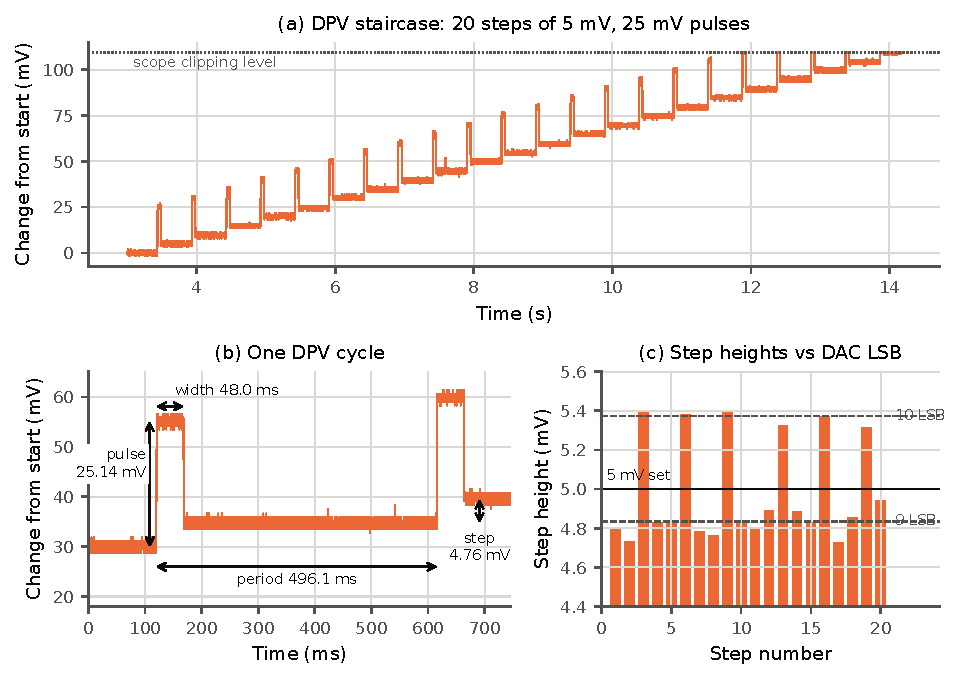
\includegraphics[width=0.78\textwidth]{figures/Testing/waveform.pdf}
\end{figure}


\subsection{Amplitude}
\label{sec:waveform_amplitude}

Every step is either \SI{4.76}{\milli\volt} or \SI{5.37}{\milli\volt} and never
deviates as illustrated in Figure~\ref{fig:waveform}c. These are 9 and
10 codes of the 12-bit DAC that sets the cell potential \cite{ad5941_ds}. A \SI{5}{\milli\volt} step is 9.31
LSB, so the firmware rounds each level to the nearest code, and the steps follow
the pattern 9, 9, 10 with a mean of \SI{4.98}{\milli\volt}. Because each level
is computed from its absolute target rather than by adding steps, the rounding
does not accumulate. The pulse is rounded to 47 LSB (\SI{25.25}{\milli\volt})
and measures \SI{25.17}{\milli\volt}. The difference between the two step
sizes, \SI{0.545}{\milli\volt}, matches the LSB to within the
\SI{\pm 3}{\percent} gain accuracy of the oscilloscope \cite{siglent_sds1000xe},
which limits how precisely the amplitudes can be verified. The applied
potential is therefore correct to within one LSB. A \SI{0.54}{\milli\volt} resolution is more than enough for DPV, where a peak is normally
about \SI{90}{\milli\volt} wide \cite{bard2001}.

\subsection{Timing}
\label{sec:waveform_timing}

The edges settle in less than \SI{0.1}{\milli\second}, which is negligible
against the \SI{50}{\milli\second} pulse. The pulse width alternates between
\SI{48.0}{\milli\second} and \SI{49.1}{\milli\second}, and the period between
two values about \SI{1}{\milli\second} apart, consistent with the
\SI{1}{\milli\second} resolution of the firmware timer. Both are shorter than
set, the pulse by \SI{1.5}{\milli\second} on average
(\SI{3}{\percent}) and the period by \SI{3.5}{\milli\second}
(\SI{0.7}{\percent}).

Timing does not affect the peak potential, which identifies the compound, so
these errors change only the peak height. For a diffusion-limited current,
which decays as $t^{-1/2}$ \cite{bard2001}, sampling \SI{3}{\percent} early
raises the measured current by about \SI{1.5}{\percent}, and the
\SI{1.1}{\milli\second} alternation varies it by about \SI{1}{\percent}
between points. The device therefore applies the programmed waveform, with
amplitudes correct to one LSB and timing within \SI{3}{\percent}. With
the excitation verified, the next check is the current it measures.

\begin{table}[H]
  \centering
  \small
  \caption{Measured excitation waveform against the programmed values.}
  \label{tab:waveform}
  \begin{tabular}{@{}l r r r@{}}
    \toprule
    \textbf{Parameter} & \textbf{Set} & \textbf{Measured} & \textbf{Error} \\
    \midrule
    Step height (20 steps)   & \SI{5}{\milli\volt}     & \SI[separate-uncertainty=true]{4.98 \pm 0.26}{\milli\volt}  & $-0.3$\,\% \\
    Pulse height (17 pulses) & \SI{25}{\milli\volt}    & \SI[separate-uncertainty=true]{25.17 \pm 0.08}{\milli\volt} & $+0.7$\,\% \\
    Pulse width              & \SI{50}{\milli\second}  & \SI[separate-uncertainty=true]{48.5 \pm 0.6}{\milli\second}  & $-3.0$\,\% \\
    Period                   & \SI{500}{\milli\second} & \SI[separate-uncertainty=true]{496.5 \pm 0.6}{\milli\second} & $-0.7$\,\% \\
    Edge time (10--90\,\%)   & --                      & $<$\SI{0.1}{\milli\second}                                 & -- \\
    \bottomrule
  \end{tabular}
\end{table}

% =====================================================================
\section{Resistor Calibration}
\label{sec:rtia_cal}

The firmware converts the high-speed TIA output to a current using the value of
the selected gain resistor $R_\text{TIA}$ \cite{ad5941_ds}, so any difference
between the nominal and the actual gain of the signal chain appears directly as
a current error. Each of the eight ranges was therefore calibrated separately.

A Plusivo DM101 digital multimeter~\cite{plusivo_dm101} was used to measure a resistor $R$, which
was connected in place of the cell. On its 2\,V DC range the multimeter has a resolution of 1\,mV
and an accuracy of $\pm0.5\,\%$, and on its 2\,k$\Omega$ to
200\,k$\Omega$ resistance ranges an accuracy of $\pm0.8\,\%$. The value of $R$ was
chosen so that $\pm0.5$\,V drives a current near the top of its operational range. At $\pm0.5$\,V
the multimeter was used to measure the voltage $V$ across the resistor, giving the true current
$I_\text{true} = V/R$, and the firmware reading $I_\text{meas}$ was recorded. Denoting the two operating points by the subscripts $+$ and $-$, a linear correction is fitted through them:
\begin{equation}
  I_\text{true} = k\,I_\text{meas} + c,
  \qquad
  k = \frac{I_{\text{true},+} - I_{\text{true},-}}{I_{\text{meas},+} - I_{\text{meas},-}},
  \qquad
  c = I_{\text{true},+} - k\,I_{\text{meas},+},
  \label{eq:rtia_cal}
\end{equation}
where the gain $k$ corrects the scale and the offset $c$ the zero. The two
points lie at opposite ends of the range, so the slope can be estimated
accurately. The correction was verified at $+\SI{0.25}{\volt}$, a point not
used in the fit.

Before calibration, $I_\text{meas}$ exceeded $I_\text{true}$ by \SIrange{9}{12}{\percent} on all
eight ranges (Table~\ref{tab:rtia_cal_tbl}). An error of the same size and sign on ranges with
different resistors points to a cause shared by the conversion chain, such as
the assumed ADC reference or PGA gain, rather than to the tolerance of the external resistors, although the internal gain resistors of the AD5941 may also share a common process error. After
correction the maximum error is \SI{0.44}{\percent}.

\begin{table}[!htbp]
  \centering
  \small
  \setlength{\aboverulesep}{0pt}
  \setlength{\belowrulesep}{0pt}
  \renewcommand{\arraystretch}{1.2}
  \caption{Two-point calibration of the high-speed TIA ranges, recomputed from
    the recorded readings. Errors are measured at $+\SI{0.25}{\volt}$.}
  \label{tab:rtia_cal_tbl}
  \begin{tabular}{@{}l r r | r | r r@{}}
    \toprule
    \textbf{Range} & \textbf{$R$ (DMM)} & \textbf{Gain $k$} & \textbf{Offset $c$ (nA)}
      & \textbf{Error before (\%)} & \textbf{Error after (\%)} \\
    \midrule
    \SI{200}{\ohm}       & \SI{994}{\ohm}         & 0.9013 & 160.0   & 11.36 & $+0.44$ \\
    \SI{1}{\kilo\ohm}    & \SI{994}{\ohm}         & 0.9141 & 278.7   &  9.70 & $+0.40$ \\
    \SI{5}{\kilo\ohm}    & \SI{4.59}{\kilo\ohm}   & 0.9089 & $-69.5$ &  9.99 & $-0.16$ \\
    \SI{10}{\kilo\ohm}   & \SI{9.93}{\kilo\ohm}   & 0.8971 & $-81.6$ & 11.78 & $-0.05$ \\
    \SI{20}{\kilo\ohm}   & \SI{19.9}{\kilo\ohm}   & 0.9018 & $-15.8$ & 11.09 & $+0.06$ \\
    \SI{40}{\kilo\ohm}   & \SI{38.5}{\kilo\ohm}   & 0.9129 & $-9.2$  &  9.72 & $+0.02$ \\
    \SI{80}{\kilo\ohm}   & \SI{81.5}{\kilo\ohm}   & 0.9158 & $-3.0$  &  9.44 & $+0.13$ \\
    \SI{160}{\kilo\ohm}  & \SI{146.7}{\kilo\ohm}  & 0.9191 & $1.1$   &  9.15 & $+0.38$ \\
    \bottomrule
  \end{tabular}
\end{table}

With the gain of every range corrected and checked against an independent
reference, the current scale of the device is known to within about
$\pm$\SI{1}{\percent}, limited by the multimeter used as the reference. This is crucial from an application perspective because the drug concentration is calculated
directly from the peak current. The next test uses Randles circuits and adds a capacitive load to the system.

% =====================================================================
\section{Randles Circuit Test}
\label{sec:randles_test}

The next test adds the capacitance of the cell. A real electrode has a
double-layer capacitance, which the DPV sampling of Section~\ref{sec:dpv_rejection} is designed
to reject. The Randles test checks this with passive networks of known DC
resistance in place of the cell \cite{c5}. A total of 7 test cells were used, three cells of the PalmSens4 dummy cell (WE~A to~C) and four networks built for this project (Cells~1 to~4), each scanned on both instruments. Once the capacitors have charged, the
DPV current depends only on the DC path, so the expected value is
$\Delta I = \Delta E_\text{pulse}/(R_s + R_{ct})$ with
$\Delta E_\text{pulse} = \SI{25}{\milli\volt}$, and zero for the networks with a
series capacitor (WE~A and Cell~2). The mean $\Delta I$ over the scan was
compared with this value, and the noise was taken as the standard deviation
(Table~\ref{tab:randles}).

\begin{table}[!htbp]
  \centering
  \footnotesize
  \setlength{\tabcolsep}{3pt}
  \caption{Ferricyanide DPV scans. Measured on its own drop, \SIrange{0.8}{1.3}{\volt}}
  \label{tab:randles}
  \begin{tabular}{@{}l l r r r r r r@{}}
    \toprule
    & & \textbf{Expected} & \multicolumn{2}{c}{\textbf{Mean $\Delta I$ (nA)}}
      & \multicolumn{2}{c}{\textbf{Error (\%)}} & \textbf{Noise (nA)} \\
    \cmidrule(lr){4-5}\cmidrule(lr){6-7}
    \textbf{Cell} & \textbf{Network} & \textbf{(nA)} & \textbf{PS4} & \textbf{\devname}
      & \textbf{PS4} & \textbf{\devname} & \textbf{PS4 / \devname} \\
    \midrule
    WE A   & $560\,\Omega + (33\,\text{nF} \parallel \text{diodes})$ & 0      & 0.00   & 0.01   & --      & --      & 0.10 / 0.07 \\
    WE B   & $10\,\text{k}\Omega$                                     & 2500.0 & 2504.4 & 2511.0 & $+0.18$ & $+0.44$ & 6.0 / 8.2 \\
    WE C   & $560\,\Omega + (33\,\text{nF} \parallel 10\,\text{k}\Omega)$ & 2367.4 & 2372.0 & 2380.5 & $+0.19$ & $+0.55$ & 5.4 / 6.1 \\
    Cell 1 & $93.8\,\text{k}\Omega$                                   & 266.5  & 264.9  & 269.7  & $-0.62$ & $+1.19$ & 2.2 / 0.8 \\
    Cell 2 & $9.83\,\text{k}\Omega + 470\,\text{nF}$                  & 0.05   & 0.11   & 0.21   & --      & --      & 0.38 / 0.09 \\
    Cell 3 & $556\,\Omega + (97.5\,\text{k}\Omega \parallel 1\,\mu\text{F})$ & 255.0 & 254.9 & 259.7 & $-0.02$ & $+1.88$ & 1.0 / 1.4 \\
    Cell 4 & $556\,\Omega + (923\,\text{k}\Omega \parallel 1\,\mu\text{F})$  & 32.4  & 33.1  & 32.4  & $+2.04$ & $-0.08$ & 0.7 / 1.2 \\
    \bottomrule
  \end{tabular}
\end{table}


Both instruments measured every network with a DC path to within
\SI{2.1}{\percent} of the expected value. The \devname{} read slightly high on
all of them except Cell~4, by \SIrange{0.4}{0.6}{\percent} on the
\SI{2.5}{\micro\ampere} networks and \SIrange{1.2}{1.9}{\percent} on the
\SI{260}{\nano\ampere} networks. The
blocking networks WE~A and Cell~2 read below \SI{0.25}{\nano\ampere} on both
instruments, so the charging current is rejected and there is no DC leakage
path. The noise on these two networks, \SIrange{0.07}{0.09}{\nano\ampere}, is the floor of the instrument itself; with the estimate of Section~\ref{sec:dpv_applications}, its $3\sigma$ of about \SI{0.25}{\nano\ampere} corresponds to roughly \SIrange{1}{5}{\micro\gram\per\litre} of efavirenz.

\begin{figure}[H]
  \caption{DPV scans of the dummy cell WE~C (Left) and Cell~3 (Right) from \SIrange{0.8}{1.3}{\volt}.}
  \label{fig:randles_curves}
  \centering
  \begin{minipage}[t]{0.49\textwidth}
    \centering
    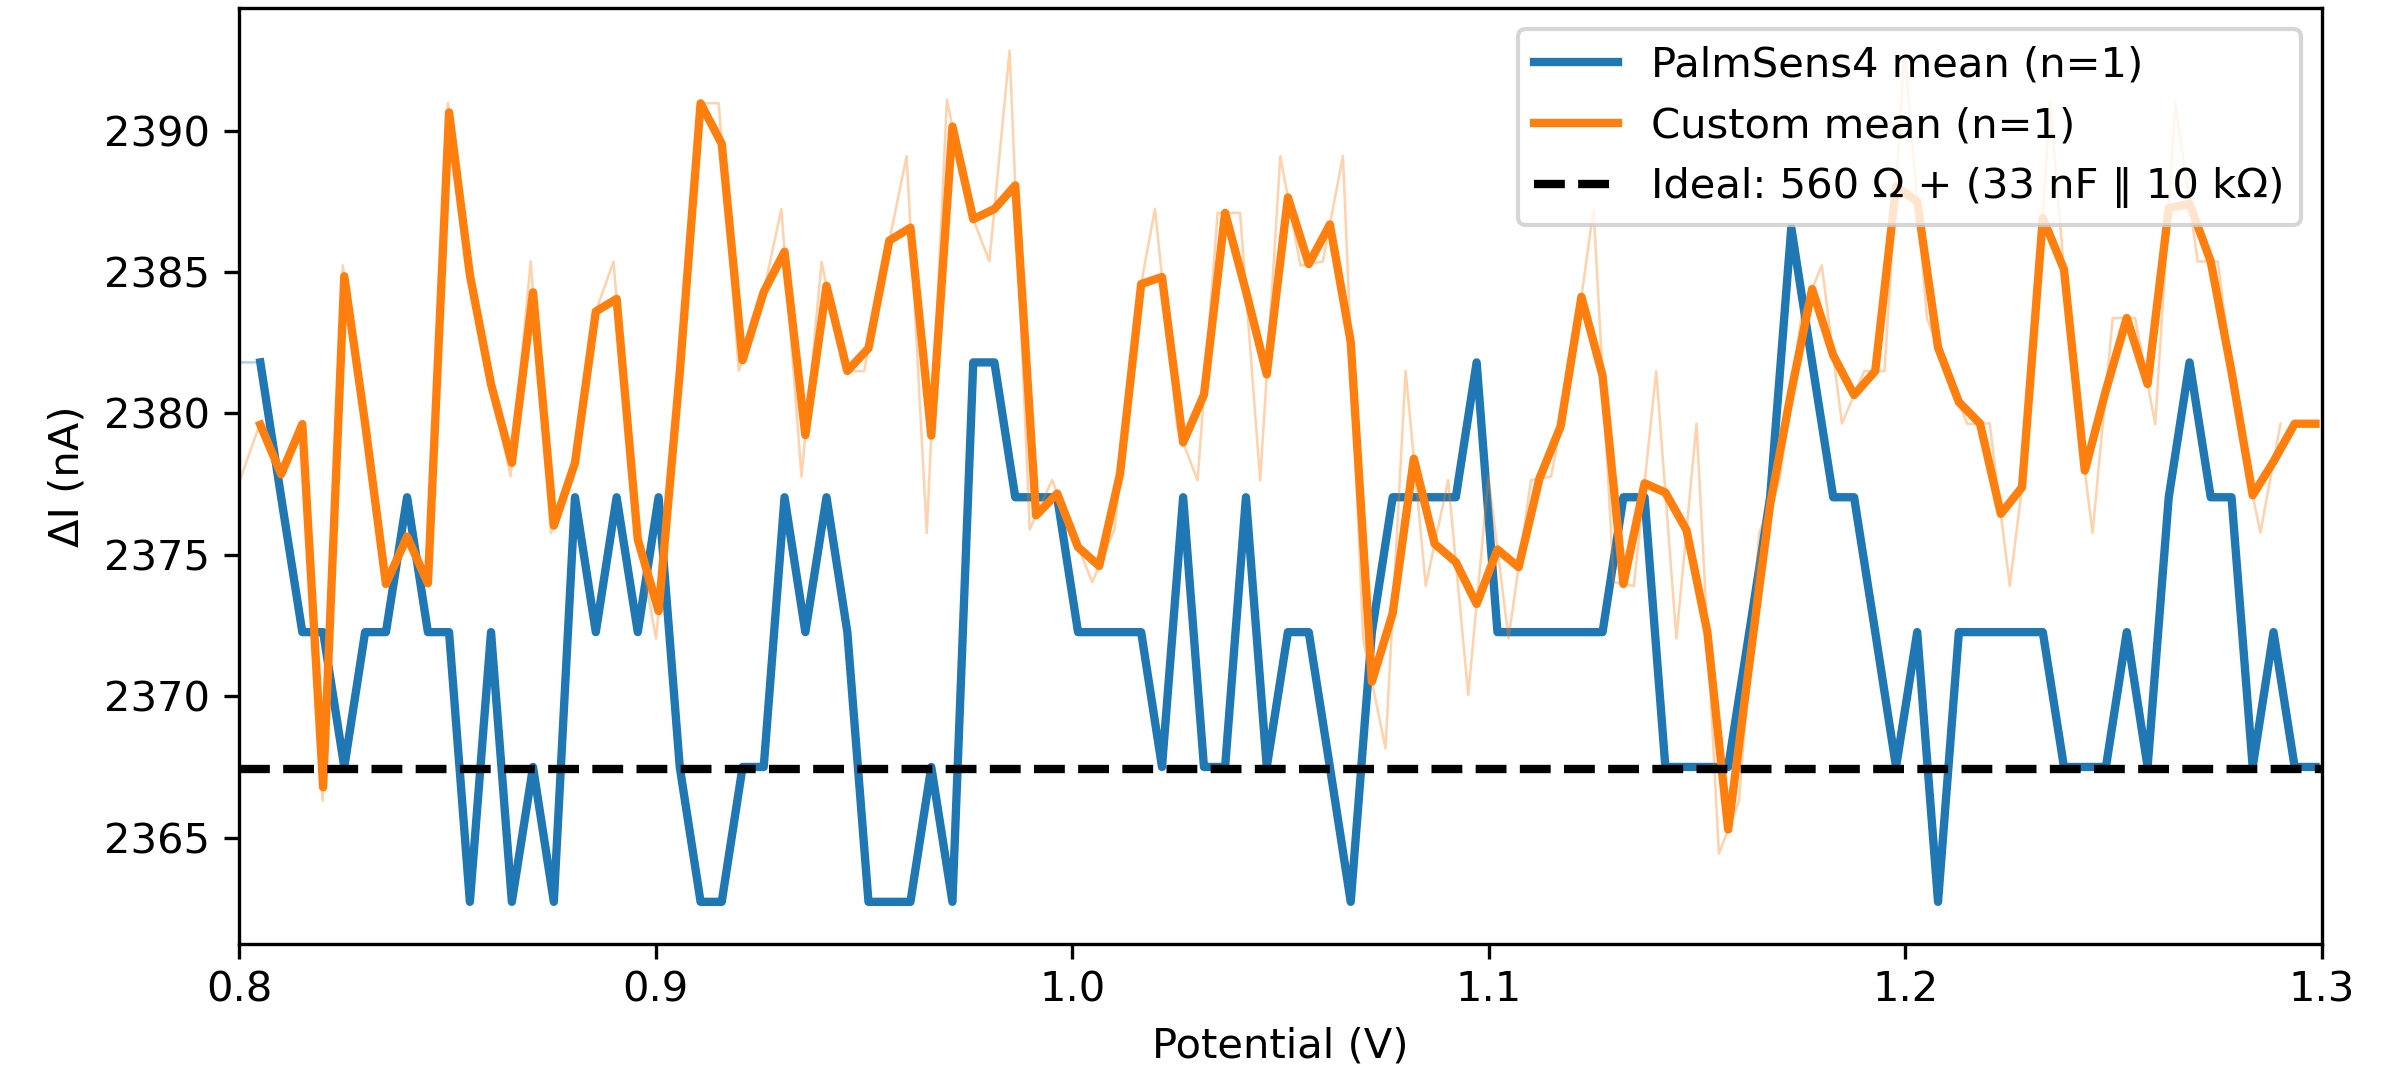
\includegraphics[width=\textwidth]{figures/Testing/randles_wec_top.png}
  \end{minipage}\hfill
  \begin{minipage}[t]{0.49\textwidth}
    \centering
    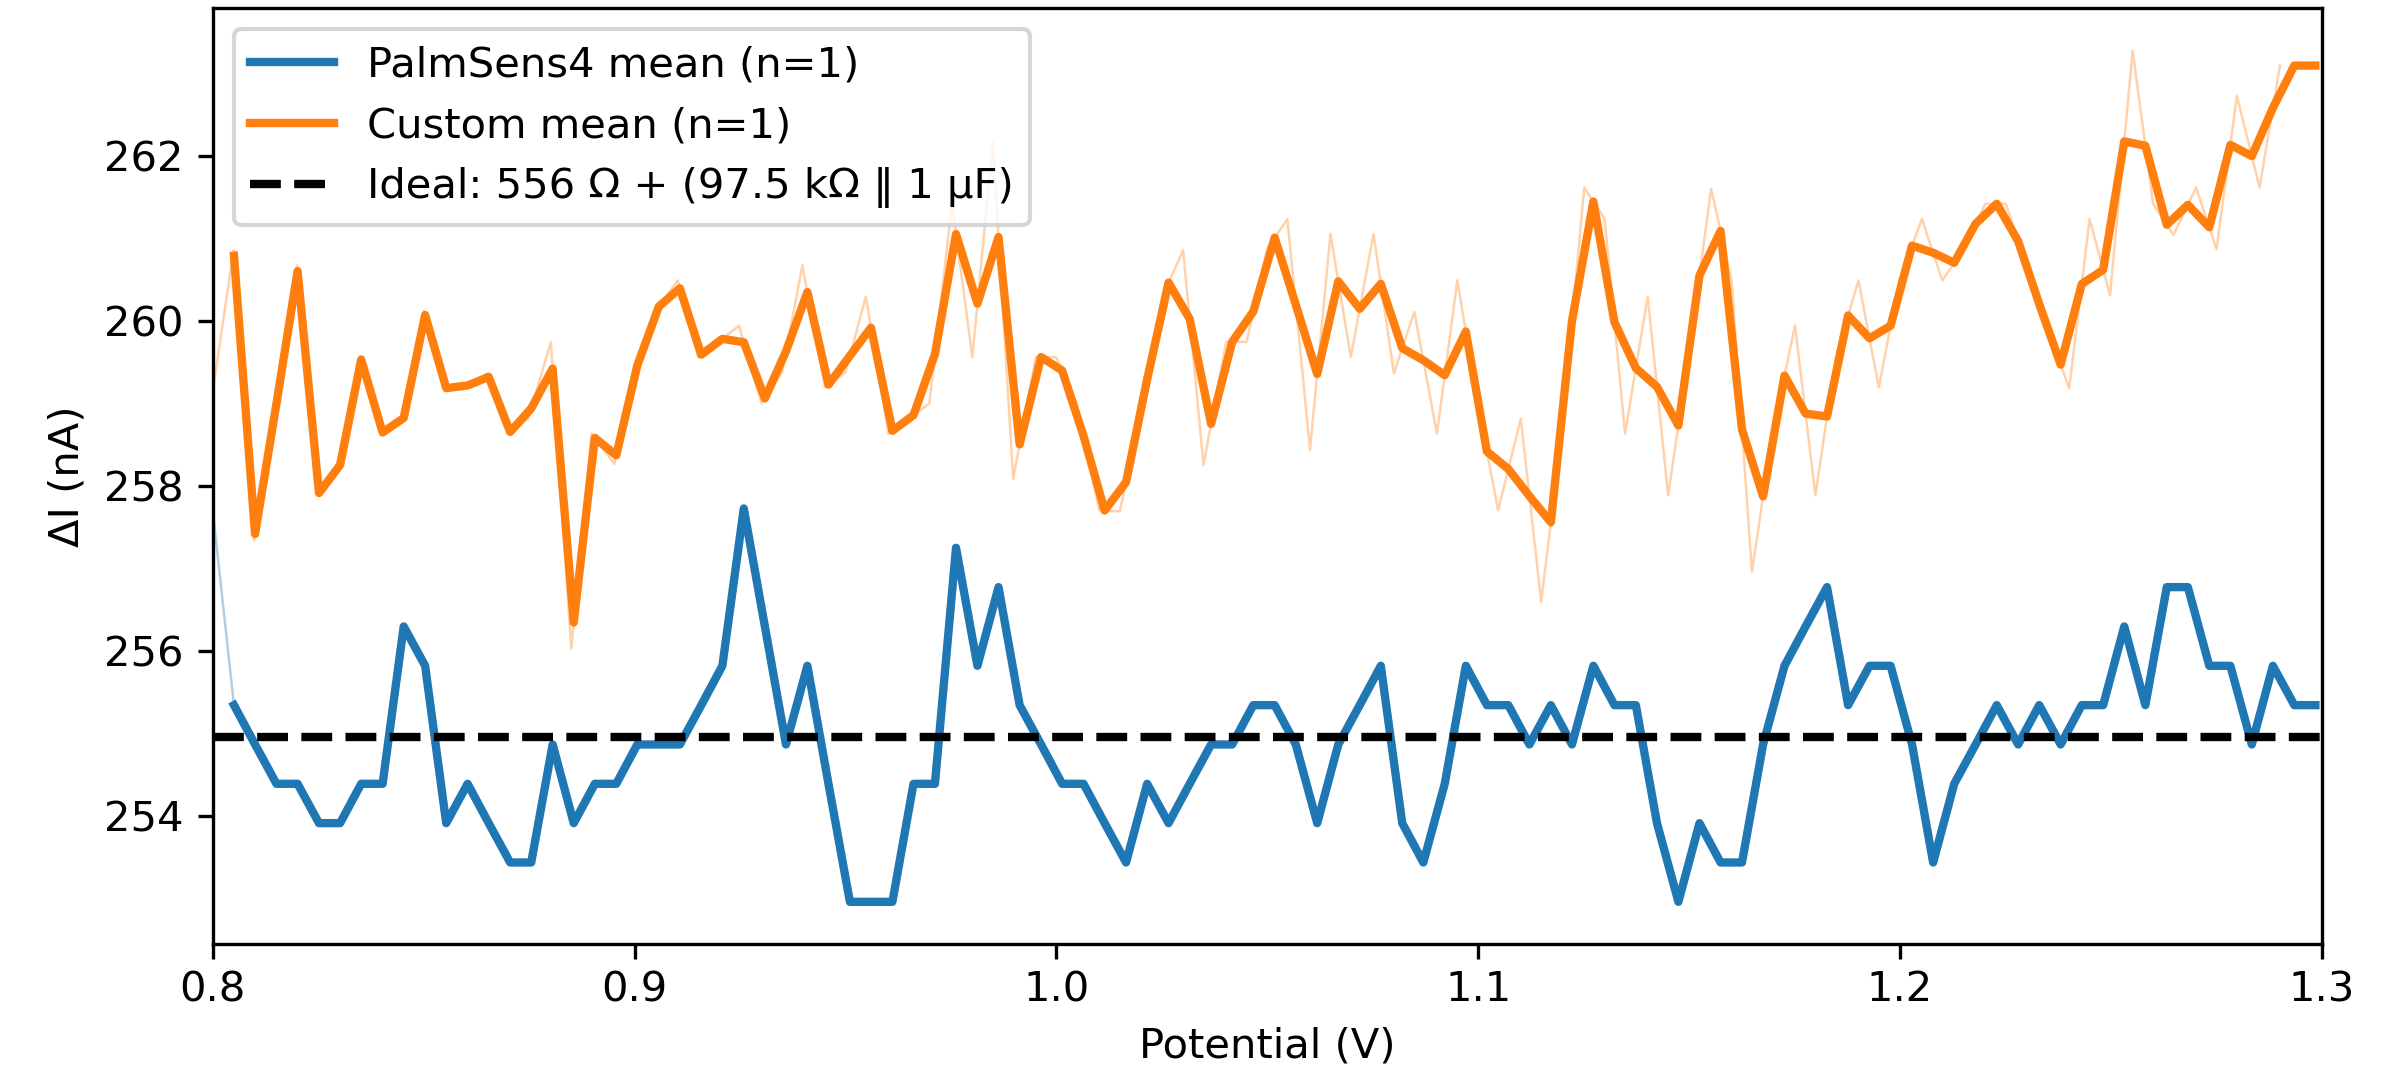
\includegraphics[width=\textwidth]{figures/Testing/randles_cell3_top.png}
  \end{minipage}
\end{figure}

The next two tests replace the known load with a real electrode. From this
point the true value is no longer known, so the PalmSens4 becomes the
reference, and its own scan-to-scan variation becomes a variable.

% =====================================================================
\section{Salt Solution Test}
\label{sec:salt_test}

The fourth test replaces the passive circuit with a real electrode. A drop of
\SI{0.1}{\Molar} KCl on the SPE has a solution resistance and a
double-layer capacitance, but no redox reaction in the scan window, which makes
it a physical Randles cell with a very large charge-transfer resistance
\cite{bard2001}. Figure~\ref{fig:pair}b shows the setup used for the salt blank tests. It should give a smooth background without a peak. The
\devname{} is judged against the PalmSens4 measuring the same solution with the
same waveform parameters.

Five pairs of salt were compared, Salt~1 to~5 as seen in Figure~\ref{fig:salt_pairs}, each consisting of one scan on each instrument on the same drop. Table~\ref{tab:salt} compares each pair quantitatively, using the mean current, the RMS difference and the correlation between the two voltammograms. The comparison runs from \SI{0.40}{\volt} to \SI{-0.20}{\volt}, so that the ferricyanide peak of Section~\ref{sec:fc_test} lies in the window.

\begin{figure}[H]
\caption{Salt solution measured by each potentiostat.}
  \label{fig:salt_pairs}
  \centering
  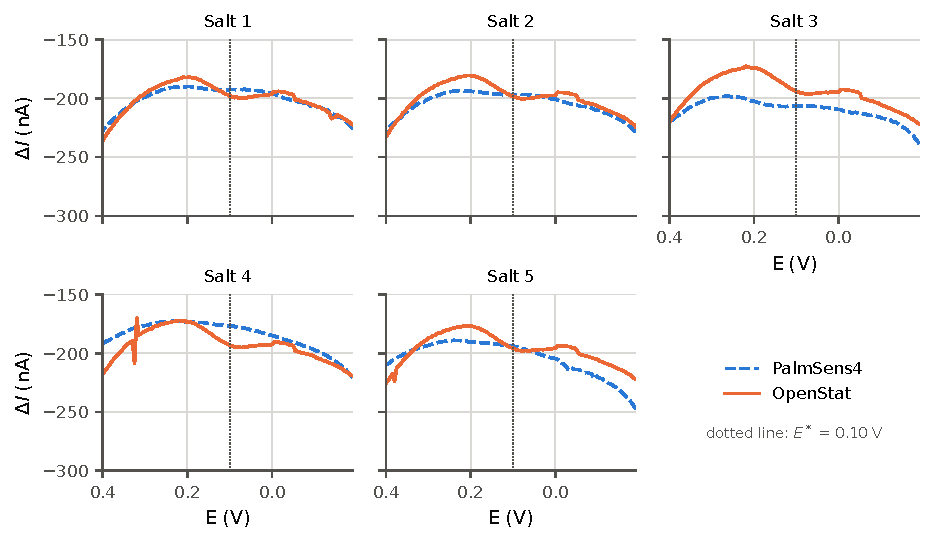
\includegraphics[width=0.7\textwidth]{figures/Testing/salt_pairs}
\end{figure}

\begin{table}[H]
  \centering
  \small
\caption{Salt test. All scans on the OpenStat used the
  $\SI{80}{\kilo\ohm}$ range. $r$ is the correlation coefficient between the PS4 and
  OpenStat voltammograms of each pair.}
    \label{tab:salt}
  \begin{tabular}{@{}l r r r r r r@{}}
    \toprule
    & \multicolumn{2}{c}{\textbf{Mean $\Delta I$ (nA)}} & \textbf{Dev.}
      & \textbf{RMS} & \textbf{Noise (nA)} & \\
    \cmidrule(lr){2-3}
    \textbf{Pair} & \textbf{PS4} & \textbf{\devname}
      & \textbf{(\%)} & \textbf{(nA)} & \textbf{PS4 / \devname} & \textbf{$r$} \\
    \midrule
    Salt 1 & $-200.7$ & $-200.0$ & $-0.3$ & 4.5  & 0.6 / 0.9 & 0.94 \\
    Salt 2 & $-204.0$ & $-199.3$ & $-2.3$ & 6.6  & 0.6 / 0.8 & 0.93 \\
    Salt 3 & $-209.6$ & $-194.0$ & $-7.4$ & 16.8 & 0.6 / 0.8 & 0.90 \\
    Salt 4 & $-184.7$ & $-192.4$ & $+4.1$ & 10.2 & 0.5 / 3.1 & 0.86 \\
    Salt 5 & $-204.2$ & $-196.4$ & $-3.8$ & 11.7 & 0.7 / 1.1 & 0.80 \\
    \bottomrule
  \end{tabular}

\end{table}


With no analyte present the current measured varies from \SIrange{-185}{-210}{\nano\ampere} on the PalmSens4 and
\SIrange{-192}{-200}{\nano\ampere} on the \devname{} as shown in Figure~\ref{fig:salt_pairs} and 
Table~\ref{tab:salt}. The mean deviation per measured pair ranges from
\SI{-7.4}{\percent} to \SI{+4.1}{\percent} and the RMS difference from
\SIrange{4.5}{16.8}{\nano\ampere}. This is larger than in the Randles test, but is of similar size as the variation of the cell itself. This is shown from scan to scan where
the PalmSens4 measurement has a standard deviation of
\SI{10.4}{\nano\ampere}, and the \devname{} \SI{3.5}{\nano\ampere}.

\section{Ferricyanide Test}
\label{sec:fc_test}
 
The last test adds a redox reaction. Ferricyanide gives a single,
well-understood reduction peak, so it tests the potential axis and the current scale together \cite{bard2001}.
\begin{equation}
  [\text{Fe(CN)}_6]^{3-} + e^- \rightleftharpoons [\text{Fe(CN)}_6]^{4-},
\end{equation}
All \devname{} scans used the \SI{1}{\kilo\ohm} range. Three
pairs were compared, FC~1 to~3, each consisting of one scan on each instrument
on a different drop as seen in Figure~\ref{fig:fc_pairs}.
 
\begin{figure}[!htbp]
  \caption{Ferricyanide DPV scans on the same drop, \devname{} run against PalmSens4 run.}
  \label{fig:fc_pairs}
  \centering
  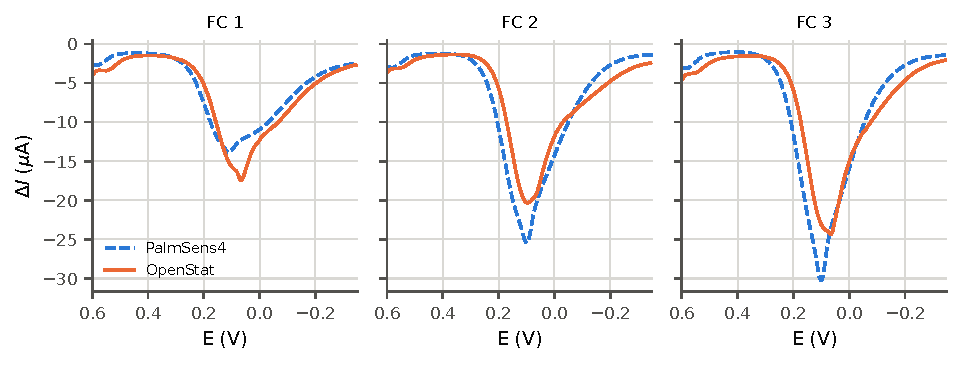
\includegraphics[width=0.8\textwidth]{figures/Testing/fc_pairs.pdf}
\end{figure}
 
The \devname{} produces a peak similar in shape to the PalmSens4 shown in its correlation $r \geq 0.956$ for
all three pairs. However, there are two visible differences: the peak heights differ by up to $\pm$\SI{26}{\percent} and the \devname{} peak lies
at a more negative potential (shifted to the right).
 
\subsection{Peak Height}
\label{sec:fc_height}
 
The peak heights of the three pairs are plotted in
Figure~\ref{fig:pair}a.
 

\begin{figure}[htbp]
  \centering
  \caption{The three ferricyanide pairs. (a) Peak height of the \devname{}
    against the PalmSens4. (b) \devname{} testing setup, either solution applied to the SPE by mechanical pipette.}
  \label{fig:pair}
  \begin{minipage}[b]{0.38\textwidth}
    \centering
    \includegraphics[width=\linewidth]{figures/testing/fc_compare_a.png}\\
    (a)
  \end{minipage}
  \hfill
  \begin{minipage}[b]{0.48\textwidth}
    \centering
    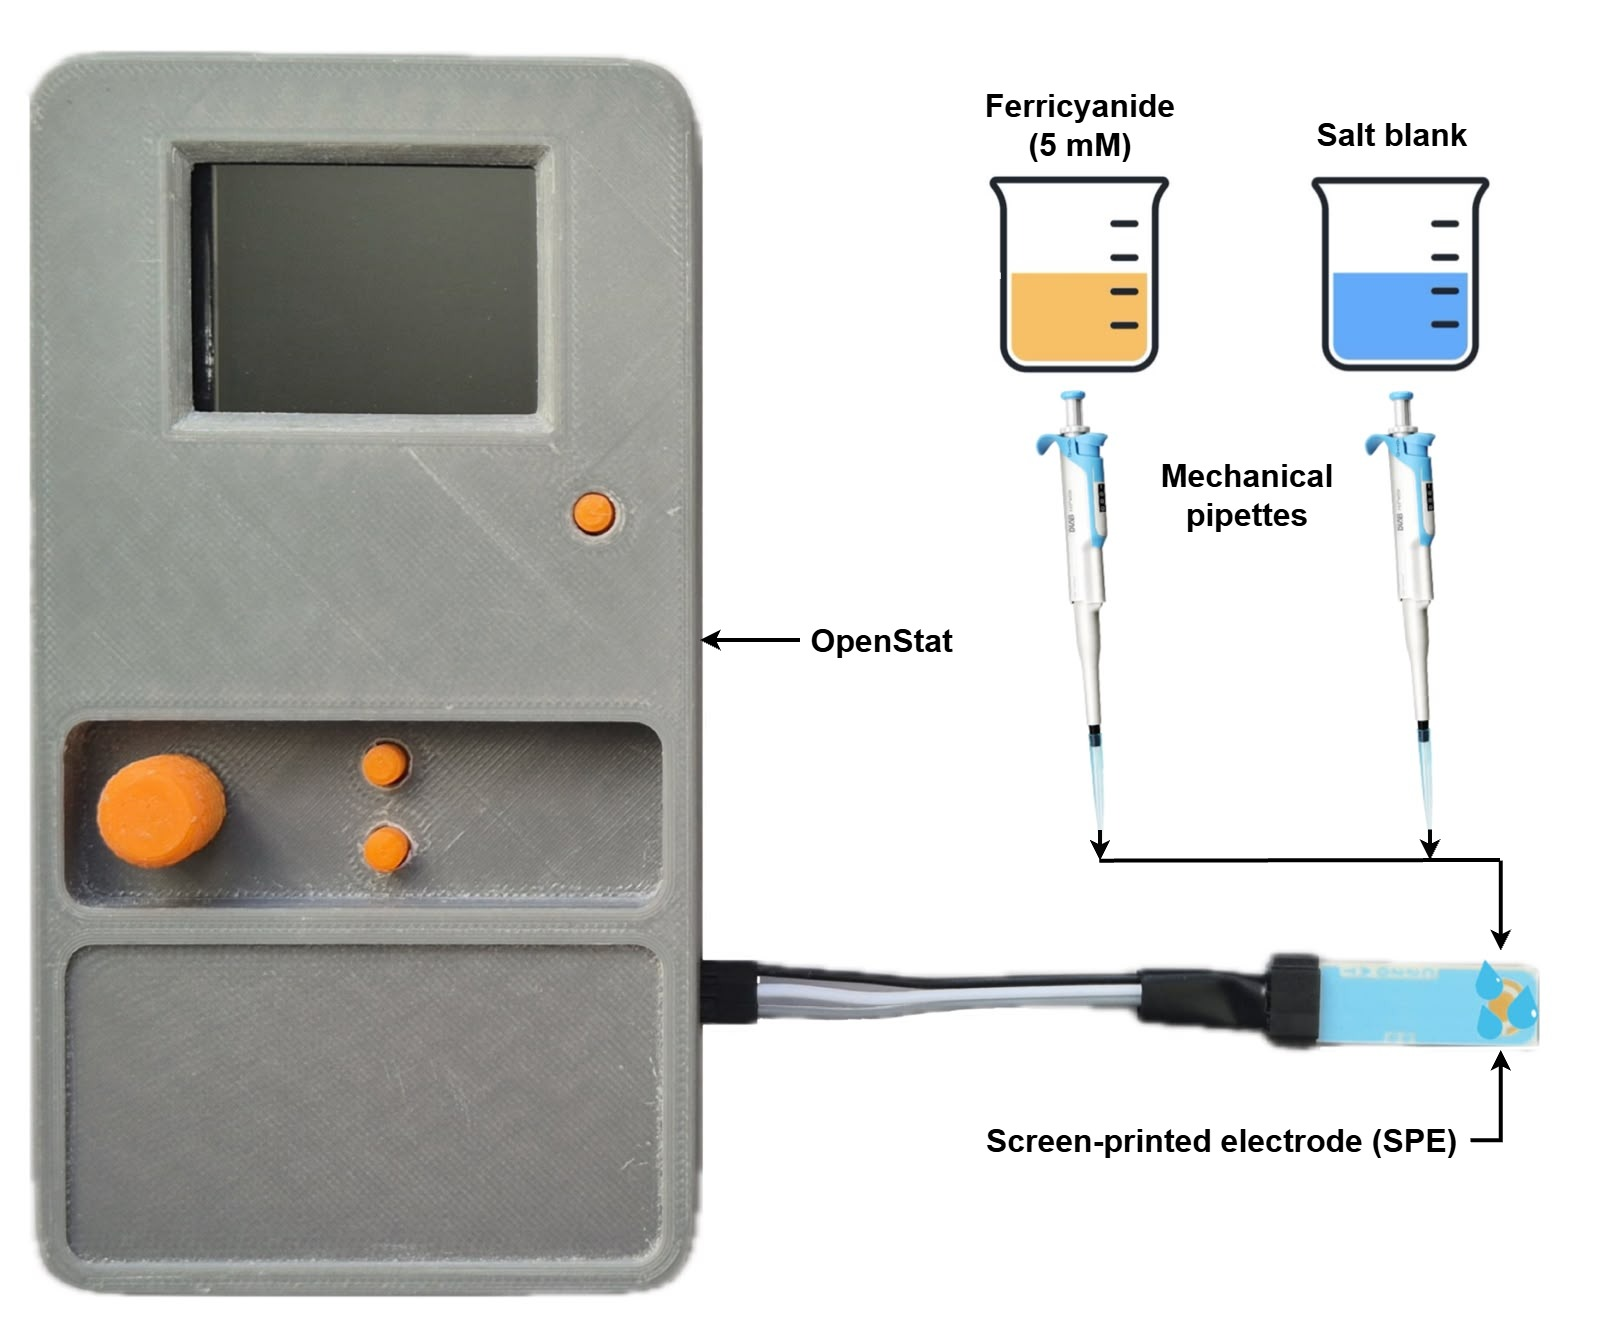
\includegraphics[width=\linewidth]{figures/testing_steps.jpg}\\
    (b)
  \end{minipage}
\end{figure}

 
The \devname{} overestimates peak height by \SI{26}{\percent} on FC~1 and underestimates it by approximately \SI{20}{\percent} on FC~2 and~3, indicating bidirectional deviation rather than regular bias. This difference must be judged against the repeatability of each instrument. Consecutive PalmSens4 scans were taken to verify this, and they vary by \SIrange{8}{52}{\percent}, while consecutive \devname{} scans vary by \SIrange{3}{33}{\percent}. The mean difference between the instruments, \SI{22}{\percent}, falls within the repeatability of the reference itself, so the test shows no instrument difference larger than the variation of the electrode, but cannot detect a smaller one. Because evaporation raises the peak over time, the later scans are expected to read higher.
 
\subsection{Peak Potential}
\label{sec:fc_shift}
 
The potential offset was found by sliding the \devname{} curve of each pair
along the potential axis until it matched the
PalmSens4 curve most closely. The offset ranges from \SIrange{20}{27.5}{\milli\volt}, where \SI{24}{\milli\volt} is the average. Shifting the \devname{} curve reduces the difference between the curves by up to a third. All the \devname{} ferricyanide scans used the \SI{1}{\kilo\ohm} range, therefore the offset
could potentially come from the specific range or its calibration. The calibration
cannot cause it, as it only rescales the current. A range-dependent cause would act through a voltage drop proportional to the
current, so the offset would grow with the peak; instead, it stays the same
while the peak more than doubles from FC~1 to FC~3
(Figure~\ref{fig:fc_pairs}). The \devname{} records each point at its base potential (Section~\ref{sec:sw_scan_flow}), and the offset is close to half of the \SI{50}{\milli\volt} pulse, which suggests that the instruments report the potential of a point at different positions within the step. Repeating a scan with a \SI{25}{\milli\volt} pulse would test this, as the offset should then halve. Until the cause is confirmed, the offset must be corrected before peak potentials are compared with published values.
 
 
\subsection{Sources of Deviation}
\label{sec:fc_deviation}
 
The remaining differences come from the solution and the testing environment, which drift between scans. Because the two instruments never measure the same drop at the same moment, this drift enters every comparison. Likely causes are:
\begin{itemize}[label=\textbullet]
  \item \textbf{Adsorption.} Gold is not inert in ferricyanide; when cyanide is 
    released from the complex and adsorbs on the gold, the gold is slowly etched. This results in the active area and electron-transfer rate to change from scan to scan \cite{vogt2016,lazar2016}. This could explain the low and varying peak currents and the movement of the peak potential.
  \item \textbf{Light sensitivity.} Ferricyanide decomposes when exposed to light; it breaks down into ferrocyanide and releases cyanide \cite{murton2025}. During every scan the drop on the electrode is exposed to room light, which lowers its ferricyanide concentration and adds cyanide that attacks the gold.
  \item \textbf{Evaporation.} A small drop loses water within minutes, which
    raises its concentration and explains why repeat scans on one drop grow in peak height rather than shrink.
\end{itemize}
The comparison would improve by using a fresh electrode for each pair,
shielding the drop from light, and starting each scan at a fixed time after the
drop is placed. 
 
\section{Summary}
\label{sec:testing_summary}
 
Table~\ref{tab:testing_summary} checks each objective of Section~\ref{sec:project_aim_obj_scope} against its target.

\begin{table}[!htbp]
  \caption{Verification of the project objectives.}
  \label{tab:testing_summary}
  \centering
  \footnotesize
  \begin{tabularx}{\textwidth}{@{}>{\raggedright\arraybackslash}p{2.0cm} >{\raggedright\arraybackslash}p{3.6cm} >{\raggedright\arraybackslash}X l@{}}
    \toprule
    \textbf{Objective} & \textbf{Target} & \textbf{Result} & \textbf{Status} \\
    \midrule
    1 Waveform   & LSB $\leq$ \SI{1}{\milli\volt}; pulse \SI{25}{\milli\volt} $\pm$ \SI{1}{\milli\volt}; period $\pm$\SI{1}{\percent}
                 & LSB \SI{0.54}{\milli\volt}; pulse \SI{25.17}{\milli\volt}; period \SI{-0.7}{\percent}; width \SI{-3}{\percent} (about \SI{1.5}{\percent} in current) & Met \\
    2 Current    & $\pm$\SI{750}{\micro\ampere}; sub-nA resolution; gain error $\leq$ \SI{1}{\percent}
                 & \SI{0.23}{\nano\ampere} per code; $\leq$ \SI{0.44}{\percent} after calibration (reference $\pm$\SI{1}{\percent}); overload at \SI{720}{\micro\ampere} in normal & Partly met \\
    3 Agreement  & Dummy cells; PalmSens4 within its repeatability
                 & Dummy cells within \SI{1.9}{\percent}; salt and ferricyanide within PalmSens4 repeatability; \SI{24}{\milli\volt} offset & Partly met \\
    4 Interfaces & Standalone and web browser operation
                 & Both demonstrated (Figure~\ref{fig:interface}, Section~\ref{sec:sw_scan_flow}) & Met \\
    5 Battery    & At least \SI{8}{\hour}
                 & \SIrange{18}{24}{\hour}, estimated from measured current (Section~\ref{sec:hw_battery}) & Met (estimate) \\
    6 Cost       & Report and compare
                 & R2\,226 incl.\ VAT (Appendix~\ref{app:bom}), against approximately R55\,400 for the PalmSens4 & Met \\
    \bottomrule
  \end{tabularx}
\end{table}

The bench tests confirm the electronics. The electrochemical comparisons were limited by the repeatability of the electrode rather than the instrument, and the \SI{24}{\milli\volt} offset remains to be explained.
